\section{EVM Contracts}
\label{sec:evm-contracts}

\subsection{Overview}

PoAI deploys a suite of smart contracts on each EVM chain for mining reward management, token operations, and market functionality.

\subsection{Contract Architecture}

\begin{center}
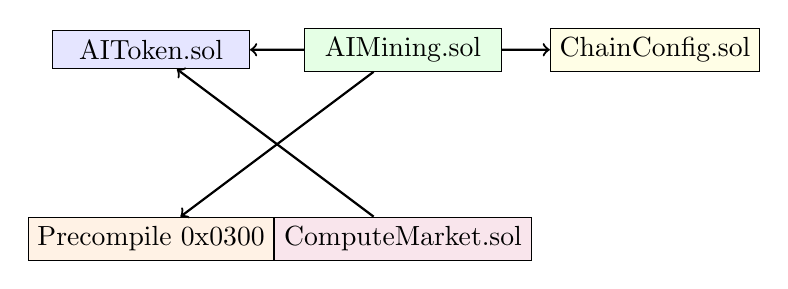
\begin{tikzpicture}[scale=0.8]
    \node[draw, rectangle, fill=blue!10, minimum width=2.5cm] (token) at (0,3) {AIToken.sol};
    \node[draw, rectangle, fill=green!10, minimum width=2.5cm] (mining) at (4,3) {AIMining.sol};
    \node[draw, rectangle, fill=yellow!10, minimum width=2.5cm] (config) at (8,3) {ChainConfig.sol};
    \node[draw, rectangle, fill=purple!10, minimum width=2.5cm] (market) at (4,0) {ComputeMarket.sol};
    \node[draw, rectangle, fill=orange!10, minimum width=2.5cm] (precompile) at (0,0) {Precompile 0x0300};

    \draw[->, thick] (mining) -- (token);
    \draw[->, thick] (mining) -- (config);
    \draw[->, thick] (market) -- (token);
    \draw[->, thick] (mining) -- (precompile);
\end{tikzpicture}
\end{center}

\subsection{AIToken.sol}

ERC20 token with mining-based minting:

\begin{lstlisting}[style=solidity]
contract AIToken is ERC20, AccessControl {
    uint256 public constant MAX_SUPPLY = 1_000_000_000 * 1e18;
    uint256 public constant HALVING_INTERVAL = 210_000;
    uint256 public constant INITIAL_REWARD = 50 * 1e18;
    uint256 public constant TREASURY_RATE = 200; // 2%

    uint256 public totalMinted;
    uint256 public genesisBlock;
    address public treasury;

    function mintReward(
        address miner,
        uint256 amount
    ) external onlyRole(MINER_ROLE) {
        require(totalMinted + amount <= MAX_SUPPLY, "Supply cap");

        uint256 treasuryAmount = amount * TREASURY_RATE / 10000;
        uint256 minerAmount = amount - treasuryAmount;

        _mint(miner, minerAmount);
        _mint(treasury, treasuryAmount);
        totalMinted += amount;

        emit RewardMinted(miner, minerAmount, currentEpoch());
    }

    function currentEpoch() public view returns (uint256) {
        return (block.number - genesisBlock) / HALVING_INTERVAL;
    }

    function currentReward() public view returns (uint256) {
        uint256 epoch = currentEpoch();
        return INITIAL_REWARD >> epoch; // Halving
    }
}
\end{lstlisting}

\subsection{AIMining.sol}

Core mining contract for proof submission:

\begin{lstlisting}[style=solidity]
contract AIMining {
    struct WorkProof {
        bytes32 sessionId;
        bytes32 nonce;
        bytes32 gpuId;
        bytes32 computeHash;
        uint256 timestamp;
        GPUTier tier;
        bytes signature;
    }

    mapping(bytes32 => bool) public spentProofs;
    IChainConfig public config;
    IAIToken public token;

    function submitProof(
        WorkProof calldata proof
    ) external returns (uint256 reward) {
        // 1. Compute work ID
        bytes32 workId = keccak256(abi.encodePacked(
            proof.gpuId,
            proof.nonce,
            block.chainid
        ));

        // 2. Check spent set
        require(!spentProofs[workId], "Already minted");

        // 3. Verify via precompile
        require(
            IAIMiningPrecompile(PRECOMPILE).verifyMLDSA(
                proof.gpuId,
                abi.encode(proof),
                proof.signature
            ),
            "Invalid signature"
        );

        // 4. Calculate reward
        reward = calculateReward(proof);

        // 5. Mark spent and mint
        spentProofs[workId] = true;
        token.mintReward(msg.sender, reward);

        emit ProofSubmitted(msg.sender, workId, reward);
    }

    function calculateReward(
        WorkProof calldata proof
    ) public view returns (uint256) {
        uint256 baseReward = token.currentReward();
        uint256 multiplier = config.getGPUMultiplier(proof.tier);
        return baseReward * multiplier / 10000;
    }
}
\end{lstlisting}

\subsection{ChainConfig.sol}

Per-chain configuration management:

\begin{lstlisting}[style=solidity]
contract ChainConfig {
    struct Config {
        uint256 baseReward;
        uint256 halvingInterval;
        uint256 difficultyTarget;
        uint256 treasuryRate;
        mapping(GPUTier => uint256) gpuMultipliers;
    }

    mapping(uint256 => Config) public chainConfigs;

    function initializeChain(
        uint256 chainId,
        uint256 baseReward,
        uint256 treasuryRate
    ) external onlyAdmin {
        Config storage cfg = chainConfigs[chainId];
        cfg.baseReward = baseReward;
        cfg.halvingInterval = 210_000;
        cfg.treasuryRate = treasuryRate;

        // Default GPU multipliers
        cfg.gpuMultipliers[GPUTier.Consumer] = 8000;     // 0.8x
        cfg.gpuMultipliers[GPUTier.Professional] = 11000; // 1.1x
        cfg.gpuMultipliers[GPUTier.DataCenter] = 13000;   // 1.3x
        cfg.gpuMultipliers[GPUTier.Sovereign] = 15000;    // 1.5x
    }

    function getGPUMultiplier(
        GPUTier tier
    ) external view returns (uint256) {
        return chainConfigs[block.chainid].gpuMultipliers[tier];
    }
}
\end{lstlisting}

\subsection{ComputeMarket.sol}

Decentralized AI service marketplace:

\begin{lstlisting}[style=solidity]
contract ComputeMarket {
    struct Provider {
        uint256 stake;
        bytes32 modelId;
        bytes32 gpuId;
        PricingModel pricing;
        uint256 activeRequests;
        uint256 maxConcurrent;
        uint256 reputation;
    }

    struct Request {
        address user;
        address provider;
        bytes32 modelId;
        bytes32 inputHash;
        bytes32 resultHash;
        uint256 payment;
        uint256 deadline;
        RequestStatus status;
    }

    mapping(address => Provider) public providers;
    mapping(bytes32 => Request) public requests;

    function createRequest(
        bytes32 modelId,
        bytes32 inputHash,
        uint256 maxPayment,
        uint256 duration
    ) external returns (bytes32 requestId) {
        // Transfer payment to escrow
        token.transferFrom(msg.sender, address(this), maxPayment);

        requestId = keccak256(abi.encodePacked(
            msg.sender,
            modelId,
            block.timestamp
        ));

        requests[requestId] = Request({
            user: msg.sender,
            provider: address(0),
            modelId: modelId,
            inputHash: inputHash,
            resultHash: bytes32(0),
            payment: maxPayment,
            deadline: block.timestamp + duration,
            status: RequestStatus.Open
        });
    }

    function submitResult(
        bytes32 requestId,
        bytes32 resultHash
    ) external {
        Request storage req = requests[requestId];
        require(req.provider == msg.sender, "Not provider");
        require(req.status == RequestStatus.Accepted, "Not accepted");

        req.resultHash = resultHash;
        req.status = RequestStatus.Completed;

        // Release payment minus market fee
        uint256 fee = req.payment * MARKET_FEE / 10000;
        token.transfer(msg.sender, req.payment - fee);
        token.transfer(treasury, fee);
    }
}
\end{lstlisting}

\subsection{Precompile Interface}

High-performance native operations at address \texttt{0x0300}:

\begin{lstlisting}[style=solidity]
interface IAIMiningPrecompile {
    /// @notice Verify ML-DSA quantum-safe signature
    /// @param pubkey ML-DSA public key (1952 bytes for Level 3)
    /// @param message Message that was signed
    /// @param signature ML-DSA signature
    /// @return valid True if signature is valid
    function verifyMLDSA(
        bytes calldata pubkey,
        bytes calldata message,
        bytes calldata signature
    ) external view returns (bool valid);

    /// @notice Calculate reward for work proof
    /// @param workProof Encoded work proof
    /// @param chainId Target chain ID
    /// @return reward Calculated reward in neurons
    function calculateReward(
        bytes calldata workProof,
        uint64 chainId
    ) external view returns (uint256 reward);

    /// @notice Verify NVTrust GPU attestation
    /// @param receipt Attested receipt from NVTrust
    /// @param signature NVTrust signature
    /// @return valid True if attestation is valid
    function verifyNVTrust(
        bytes calldata receipt,
        bytes calldata signature
    ) external view returns (bool valid);

    /// @notice Check if work ID is in spent set
    /// @param workId Work identifier
    /// @return spent True if already minted
    function isSpent(bytes32 workId) external view returns (bool spent);

    /// @notice Compute work ID from components
    /// @param deviceId GPU device ID
    /// @param nonce Unique nonce
    /// @param chainId Target chain ID
    /// @return workId Computed work identifier
    function computeWorkId(
        bytes32 deviceId,
        bytes32 nonce,
        uint64 chainId
    ) external pure returns (bytes32 workId);
}
\end{lstlisting}

\subsection{Gas Costs}

\begin{center}
\begin{tabular}{lcc}
\toprule
\textbf{Operation} & \textbf{Precompile} & \textbf{Pure Solidity} \\
\midrule
verifyMLDSA & 3,000 gas & 500,000+ gas \\
calculateReward & 1,000 gas & 10,000 gas \\
verifyNVTrust & 5,000 gas & 1,000,000+ gas \\
isSpent & 100 gas & 2,100 gas (SLOAD) \\
computeWorkId & 50 gas & 500 gas \\
\bottomrule
\end{tabular}
\end{center}

\subsection{Deployment Addresses}

\begin{center}
\begin{tabular}{llc}
\toprule
\textbf{Contract} & \textbf{Address} & \textbf{All Chains} \\
\midrule
AIToken & 0xAI00...0001 & \checkmark \\
AIMining & 0xAI00...0002 & \checkmark \\
ChainConfig & 0xAI00...0003 & \checkmark \\
ComputeMarket & 0xAI00...0004 & \checkmark \\
Precompile & 0x0300 & \checkmark \\
\bottomrule
\end{tabular}
\end{center}
